\section{Herramientas para el desarrollo de robots}
En esta sección se presenta el sistema operativo robótico (conocido como ROS), a su vez de la herramienta de simulación Gazebo, ambas necesarias para la realización del trabajo.

\subsection{ROS}
Robot Operating System (ROS) es un \textit{framework} open source pensado para escribir software orientado a robots. El mismo cuenta con herramientas, librerías y convenciones que buscan simplificar la tarea de crear robots complejos y robustos. Desarrollado originalmente en 2007, el mismo cuenta con diferentes versiones hasta la fecha, cada una de ellas pensada para las distintas versiones estables con soporte de largo plazo (LTS, \textit{long term support}) del sistema operativo Ubuntu, aunque también se ha adaptado a otros sistemas operativos, como Arch, Debian y Microsoft Windows (considerados a muchos de ellos como versiones ''experimentales'' del framework).

Si bien existen tanto ROS como ROS2, en este trabajo se hará énfasis en el primero.

\subsubsection{Sistema ROS}
Un sistema ROS consiste de diferentes programas corriendo simultáneamente y comunicándose entre si mediante \textit{mensajes}. Estos mensajes se representan mediante una \textit{estructura de grafos}, como puede observarse en la Figura \ref{fig:rosgraph}, donde los programas que reciben o envían mensajes representan los \textit{nodos grafos}, indicando como se comunican entre sí mediante las flechas. Estos nodos suelen ser procesos POSIX, mientras que las flechas suelen ser conexiones TCP, aumentando así la tolerancia a fallos.

\begin{figure}[!ht]
    \centering
    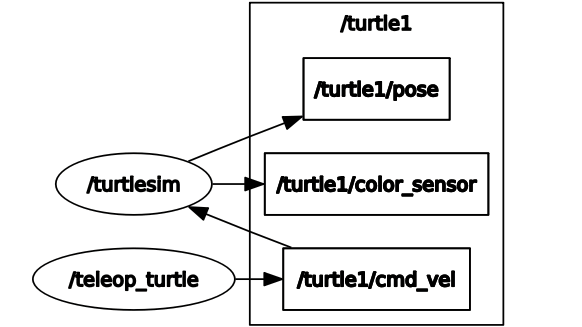
\includegraphics[width=\linewidth]{Img/ROSGraph.png}
    \caption{Ejemplo de un grafo de ROS}
    \label{fig:rosgraph}
\end{figure}

\subsubsection{\texttt{roscore}}
Si bien la comunicación entre los nodos es entre uno y otro (\textit{peer-to-peer}), los mismos necesitan conocer en todo momento aquellos nodos con los cuales se tienen que comunicar. Para resolver esto, el servicio \texttt{roscore} provee la información de conexión necesaria para que los nodos encuentren a otros. Al crearse un nuevo nodo, el mismo se conecta al \texttt{roscore} y le informa los detalles tanto de los mensajes que publica como los que pretende recibir. Por ello, cuando un nuevo nodo aparece, el \texttt{roscore} le informa lo necesario para realizar una conexión peer-to-peer con los nodos que comparten los mismos tópicos de mensajes.

Como todos los nodos deben comunicarse con el \texttt{roscore} desde el momento de su ejecución, es necesario correr primero dicha instancia en una terminal
\begin{lstlisting}[language=bash]
  $ roscore
\end{lstlisting}

\subsubsection{Estructura}
A continuación, se hará una breve descripción de la estructura de archivos ROS junto con una serie de comandos útiles. En caso que se requiera conocer más del tema como, por ejemplo, crear paquetes y workspaces, se recomienda ir a la página específica\footnote{http://wiki.ros.org/ROS/Tutorials}.

\paragraph{catkin workspace}
Antes de comenzar a escribir código ROS, es necesario generar un \textit{workspace} para que este código resida allí. Como ROS es una colección muy variada de paquetes cuyas dependencias pueden variar, para, por ejemplo, poder crear el mismo, generar ejecutables, librerías, entre otras cosas, el mismo utiliza el sistema de construcción \textit{catkin}\footnote{\url{http://wiki.ros.org/catkin}}, el cual otorga una funcionalidad extra al flujo de trabajo normal de \texttt{CMake}, tomando a este como la base del mismo. Por ello, no solo utiliza el archivo \textit{CMakelists.txt}, sino que también agrega el \textit{package.xml}. Una vez creado el mismo, la estructura de carpetas resultante es típicamente el presentado en la Figura \ref{fig:catkinworkspace}, donde, además del \textit{CMakelists.txt}, se distinguen tres subcarpetas
\begin{itemize}
    \item \textit{src}: donde se encuentra el código fuente de los distintos paquetes, detallados más adelante.
    \item \textit{build}: donde CMake se invoca para construir los paquetes catkin en el espacio src.
    \item \textit{devel}: donde los paquetes construidos se colocan antes de ser instalados.
\end{itemize}
% \begin{figure}[!ht]
%     \centering
%     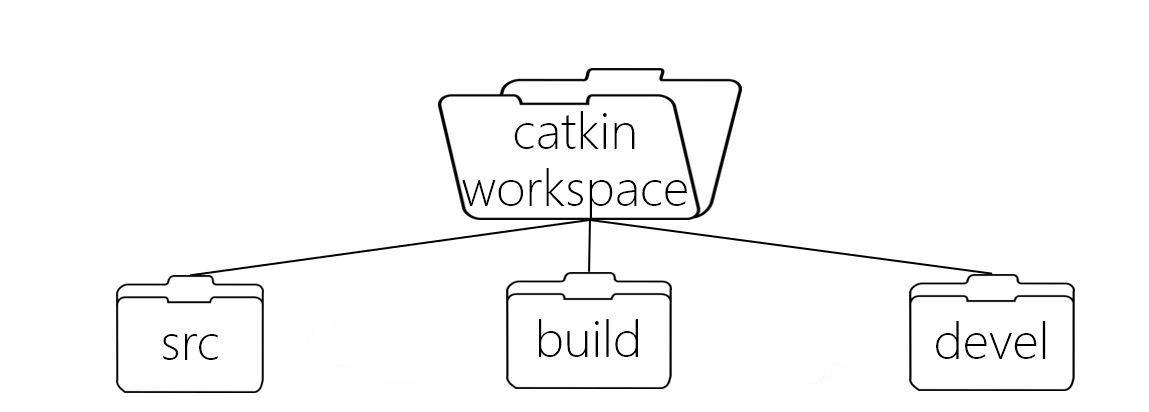
\includegraphics[width=\linewidth]{Img/CatkinWorkspace.jpeg}
%     \caption{catkin workspace típico de ROS}
%     \label{fig:catkinworkspace}
% \end{figure}
\begin{figure}[!ht]
    \centering
    \begin{forest}
    for tree={
      parent anchor=south,
      child anchor=north,
      node options={inner sep=11pt},
      l sep=50pt,
      s sep=80pt,
    } 
    [\myfolder{catkin\_ws}
      [\myfolder{src}]
      [\myfolder{build}]
      [\myfolder{devel}]
    ]
    \end{forest}
    \caption{catkin workspace típico de ROS}
    \label{fig:catkinworkspace}
\end{figure}


Una forma estándar de crear un catkin workspace es mediante el uso de \lstinline[language=bash]{catkin_make} en un directorio con la carpeta \textit{src} presente. Esta acción, además de crear las carpetas \textit{build} y \textit{devel}, proporcionará el \textit{CMakeLists.txt} correspondiente al workspace.
\begin{lstlisting}[language=bash]
$ mkdir -p ~/catkin_ws/src
$ cd ~/catkin_ws/
$ catkin_make
\end{lstlisting}

\paragraph{Paquetes}
El software de ROS está organizado en \textit{paquetes}, los cuales pueden contener dentro de ellos nodos, librerías independientes, archivos de configuración, entre otros. Estos paquetes son, entonces, una colección de recursos que se construyen y distribuyen conjuntamente, con el objetivo de proporcionar la funcionalidad requerida de una manera sencilla para que el software pueda reutilizarse fácilmente. En general, los paquetes ROS cuentan con suficiente funcionalidad para ser útil, pero no demasiado para que el paquete sea pesado y difícil de usar desde otro software. Como se mencionó anteriormente, los mismos suelen residir en la carpeta \textit{src} del \textit{catkin workspace}, pudiendo estar en un árbol de subcarpetas, como por ejemplo en la Figura \ref{fig:catkinworkspacewithpackages}.
% \begin{figure}[!ht]
%     \centering
%     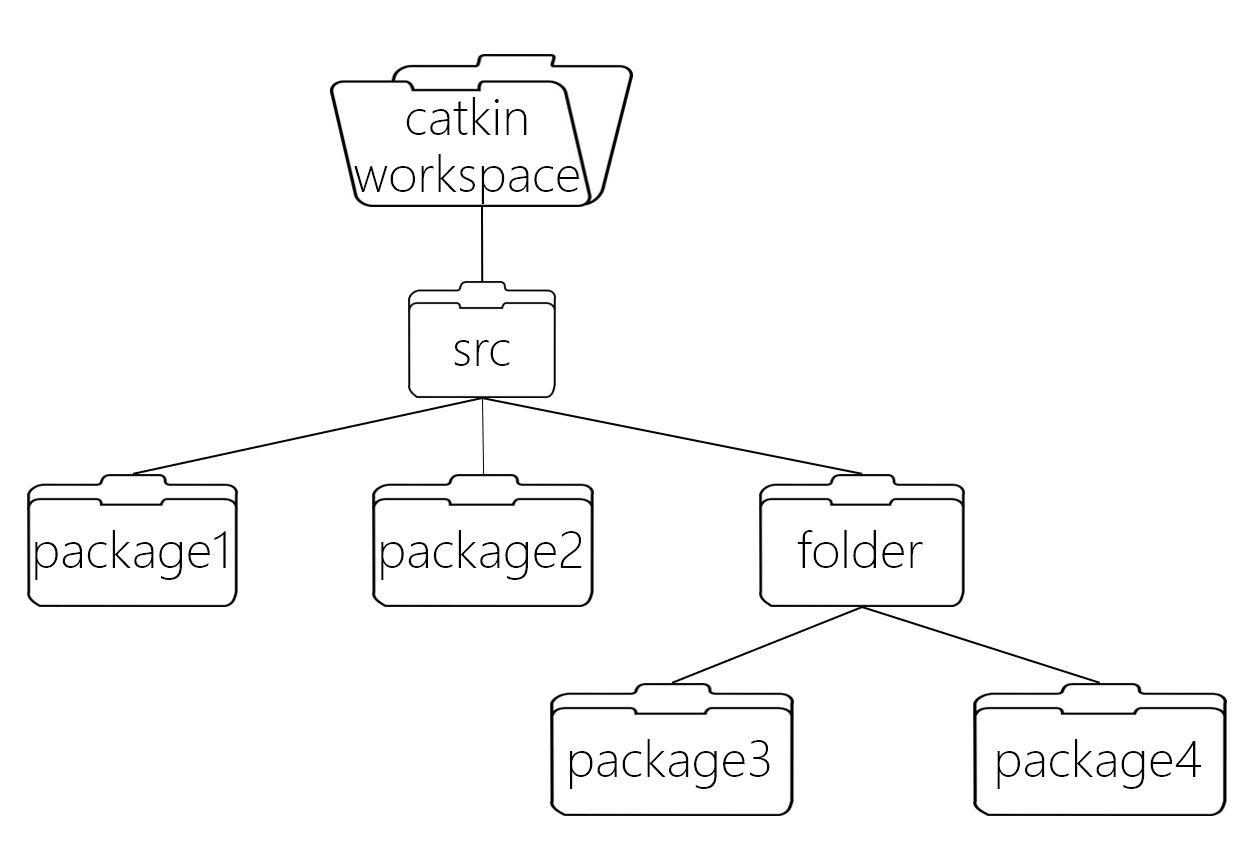
\includegraphics[width=\linewidth]{Img/CatkinWorkspaceWithPackages.jpeg}
%     \caption{Ejemplo de varios paquetes dentro de un catkin workspace}
%     \label{fig:catkinworkspacewithpackages}
% \end{figure}
\begin{figure}[!ht]
    \centering
    \begin{forest}
    for tree={
      parent anchor=south,
      child anchor=north,
      node options={inner sep=11pt},
      l sep=50pt,
      s sep=80pt,
    } 
    [\myfolder{catkin\_ws}
      [\myfolder{src}
          [\myfolder{paquete1}]
          [\myfolder{paquete2}]
          [\myfolder{carpeta}
            [\myfolder{paquete3}]
            [\myfolder{paquete4}]
          ]
      ]
    ]
    \end{forest}
    \caption{Ejemplo de varios paquetes dentro de un catkin workspace}
    \label{fig:catkinworkspacewithpackages}
\end{figure}


\subparagraph{rosrun}
Como los paquetes pueden contener una gran cantidad de ejecutables (los nodos en sí), para evitar el uso de rutas largas dentro del \textit{filesystem} para correrlos, ROS provee una utilidad a la línea de comandos denominada \texttt{rosrun}, el cual busca un programa propio de un paquete específico, además de poder proveerle parámetros. Por lo tanto, teniendo en una terminal el \texttt{roscore} ejecutándose, es posible correr un ejecutable de un paquete ROS mediante
\begin{lstlisting}[language=bash]
  $ rosrun PAQUETE EJECUTABLE [ARGS]
\end{lstlisting}

Por ejemplo, si se tiene un paquete llamado \textit{prueba}, el que implementa un programa asociado al ejecutable \textit{hola}, el mismo podría ser ejecutado mediante la sentencia
\begin{lstlisting}[language=bash]
  $ rosrun prueba hola
\end{lstlisting}

\subparagraph{roslaunch}
En caso que se requiera ejecutar una gran cantidad de nodos, abrir una terminal para cada uno de ellos puede ser tedioso, sumado a que se puede llegar a tener un gran numero de parámetros para cada uno de ellos. Para evitar este inconveniente, existe el comando \texttt{roslaunch}, el cual es similar a \texttt{rosrun} en su estructura
\begin{lstlisting}[language=bash]
  $ roslaunch NOMBRE_PAQUETE ARCHIVO_LAUNCH
\end{lstlisting}
con la diferencia de que opera sobre \textit{archivos .launch}, los cuales son archivos XML que puede poseer la descripción de una serie de nodos y parámetros, entre otras cosas.

\subsubsection{Tipos de mensajes}
ROS provee una gran cantidad de tipos de mensajes dentro de su estructura, desde tipos estándar (en \texttt{std\_msgs}\footnote{\url{http://wiki.ros.org/std_msgs}}) hasta mensajes de mayor complejidad, como puede ser mensajes de sensores específicos (en \texttt{sensor\_msgs}\footnote{\url{http://wiki.ros.org/sensor_msgs}}).

Uno de los tipos de mensajes más utilizados dentro de ROS se trata del \texttt{std\_msgs/Header}, ya que cuenta con información respecto al paso de tiempo del sistema, que se encuentra vinculado con el \texttt{roscore}. El mismo suele ser de importancia ya sea, por ejemplo, para calcular una integración temporal, o sólo para tener una noción del orden de los distintos tópicos que fue recibiendo un nodo.

Existen casos en los que los tipos de mensajes predefinidos por ROS no son suficientes. Por ello, se cuenta con la posibilidad de crear nuevos. Esto suele realizarse en la carpeta \textit{msg} dentro de un proyecto en si, y tienen como gran ventaja de ser fáciles de implementar y cortos.

\subsubsection{Tópicos}
Como se dijo anteriormente, el sistema ROS consiste en un conjunto de \textit{nodos} independientes que en su conjunto forman un \textit{grafo}. La forma más común de que los distintos nodos se comunican entre sí a través de \textit{tópicos}, los cuales son un \textit{stream de mensajes} con un tipo definido. Por ejemplo, los datos de un acelerómetro pueden enviarse en el tópico \texttt{accelerometer}, con un mensaje del tipo \texttt{Accel}. 

Estos tópicos implementan el mecanismo de comunicación de \textit{publicar/suscribir}. Para el caso de los nodos que quieren publicar información, primero deben \textit{anunciar} (\textit{advertise}) tanto el nombre del tópico como los tipos de mensaje que se enviarán al \texttt{roscore}. Una vez hecho esto, pueden empezar a \textit{publicar} (\textit{publish}) la información actual en el tópico. En cambio, los nodos que pretenden recibir mensajes de un tópico específico, primero deben \textit{suscribirse} (\textit{subscribe}) al tópico en cuestión haciendo un pedido al \texttt{roscore}. Luego de la suscripción, todos los mensajes en el tópico son entregados al nodo que hizo la petición. Un ejemplo de esto puede observarse en la Figura \ref{fig:rostopics}.
\begin{figure}
    \centering
    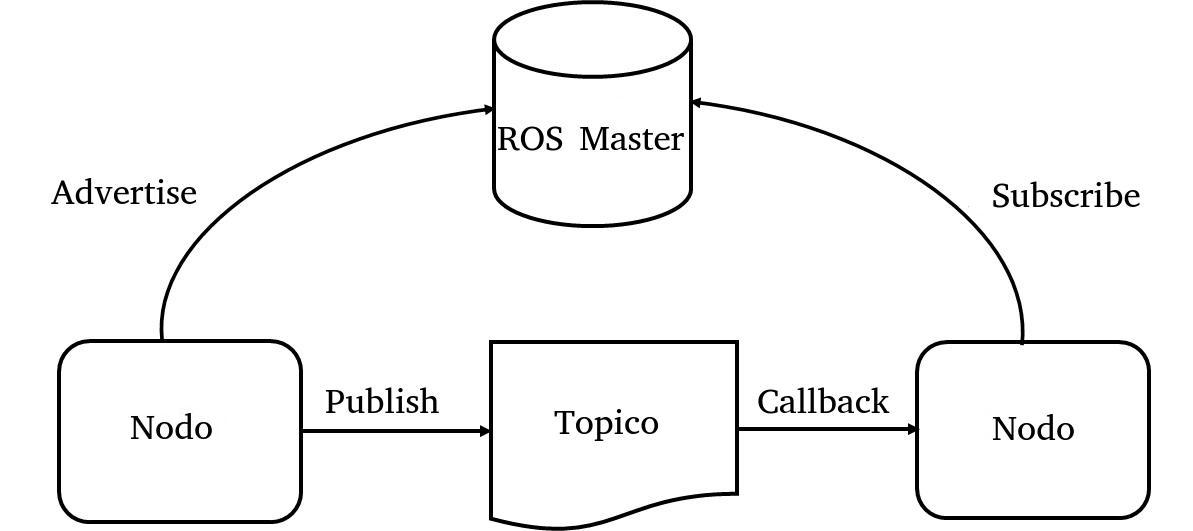
\includegraphics[width=\linewidth]{Img/ROSTopics.jpg}
    \caption{Estructura básica de un publicador/suscriptor comunicándose mediante un tópico}
    \label{fig:rostopics}
\end{figure}

Como pueden existir una gran cantidad de tópicos ejecutándose al mismo tiempo, el comando de la terminal \texttt{rostopic} es de gran ayuda para poder, por ejemplo, listar, escuchar y obtener información de los mismos.

\subsubsection{\texttt{rosbag}}
Una de las grandes ventajas que presenta ROS respecta a la posibilidad de poder grabar tópicos ROS, para luego poder reproducirlos en cualquier momento. Esto se encuentra disponible mediante el set de herramientas \texttt{rosbag}\footnote{\url{http://wiki.ros.org/rosbag}}, el cual almacena dichos datos en \textit{''bolsas''} (del término \textit{bags} en inglés), permitiendo entonces, por ejemplo, el análisis de los algoritmos utilizados sobre un mismo set de datos. El uso de archivos de bolsa dentro de ROS generalmente no es diferente de hacer que los nodos ROS envíen los mismos datos, aunque puede encontrar problemas con los datos con pasos de tiempo almacenados dentro de los datos del mensaje. Por este motivo, la herramienta \texttt{rosbag} incluye una opción para publicar un reloj simulado que corresponde a la hora en que se registraron los datos en el archivo.

\subsection{Gazebo}
Si bien no es específicamente parte de ROS (aunque si se vincula con el mismo), Gazebo\footnote{http://gazebosim.org/} es un entorno de simulación pensado principalmente para robots, lo cual es una herramienta esencial no sólo para tener un entorno controlado y poder testear los algoritmos realizados, sino también para poder estimar los valores necesarios para poder llevar a cabo una tarea específica con robots sin tener que afrontar los riesgos que generaría realizarlo experimentalmente. 

Entonces, Gazebo permite probar rápidamente algoritmos, diseñar robots, realizar pruebas de regresión y entrenar el sistema de inteligencia artificial utilizando escenarios realistas. Gazebo ofrece la capacidad de simular de forma precisa y eficiente poblaciones de robots en entornos complejos de interior y exterior. 

\subparagraph{Vinculación con ROS}
Gazebo permite publicar mediante mensajes ROS los datos que observan los sensores utilizados, permitiendo así una rápida vinculación con dicho framework. Existen, a su vez, una gran cantidad de robots que ya se encuentran preparados para operar en Gazebo, publicando los datos de los mismos en base al entorno en el que se encuentran.

\subsection{Resumen}
En esta sección se presentó una muy breve introducción a ciertos aspectos de ROS, sin entrar en detalle en la implementación a nivel usuario que debe realizarse, sino para poder tener en mente la estructura que presenta el mismo. En las secciones posteriores, a medida que se vayan desarrollando los temas se irán introduciendo paquetes de ROS que han resultado de utilidad para el desarrollo de la tesis.

A su vez, se dio una introducción a Gazebo, herramienta que será de vital importancia en la corroboración de los algoritmos realizados